\documentclass[11pt, oneside]{article}
\usepackage[letterpaper, margin=2cm]{geometry}
\usepackage{MATH565}

\begin{document}
\noindent \textbf{\Large{Caleb Logemann \\
MATH 565 Continuous Optimization \\
Final Exam
}}

%\lstinputlisting[language=Python]{H01_23.m}
\begin{enumerate}
  \item % #1 Done
    \begin{enumerate}
      \item[(a)] % Done
        \begin{proof}
          Using Taylor Series for $f$ we know that
          \[
            f(x_k + \alpha p_k) = f(x_k) + \alpha p_k^T \nabla f(tx_k + (1-t)(x_k + \alpha p_k)) 
          \]
          for some $t \in \br{0, 1}$.
          This can be simplified as follows
          \begin{align*}
            f(x_k + \alpha p_k) &= f(x_k) + \alpha p_k^T \nabla f(tx_k + (1-t)(x_k + \alpha p_k)) \\
            &= f(x_k) + \alpha p_k^T \nabla f(x_k) + \alpha p_k^T \nabla f(tx_k + (1-t)(x_k + \alpha p_k)) - \alpha p_k \nabla f(x_k) \\
            &= f(x_k) + \alpha p_k^T \nabla f(x_k) + \alpha p_k^T \p{\nabla f(tx_k + (1-t)(x_k + \alpha p_k)) - \nabla f(x_k)}
            \intertext{By Cauchy-Schwarze}
            &\le f(x_k) + \alpha p_k^T \nabla f(x_k) + \alpha \norm{p_k} \norm{\nabla f(tx_k + (1-t)(x_k + \alpha p_k)) - \nabla f(x_k)} \\
            \intertext{By the Lipschitz continuity of $\nabla f$}
            &\le f(x_k) + \alpha p_k^T \nabla f(x_k) + \alpha L \norm{p_k} \norm{tx_k + (1-t)(x_k + \alpha p_k) - x_k} \\
            &= f(x_k) + \alpha p_k^T \nabla f(x_k) + \alpha L \norm{p_k} \norm{tx_k + (1-t)x_k + (1-t)\alpha p_k - x_k} \\
            &= f(x_k) + \alpha p_k^T \nabla f(x_k) + \alpha L \norm{p_k} \norm{(1-t)\alpha p_k} \\
            &= f(x_k) + \alpha p_k^T \nabla f(x_k) + \alpha^2 (1-t) L \norm{p_k}^2 \\
            &\le f(x_k) + \alpha p_k^T \nabla f(x_k) + \alpha^2 L \norm{p_k}^2
          \end{align*}
          This establishes the desired result.
        \end{proof}

      \item[(b)] % Done
        Prove that
        \[
          \lim[k \to \infty]{\nabla f(x_k)} = 0
        \]

        \begin{proof}
          First I will show that $p_k$ is a descent direction.
          In order to do this consider $p_k^T \nabla f(x_k)$.
          \begin{align*}
            p_k^T \nabla f(x_k) &= - (\nabla f(x_k) \cdot e_{j_k})^T \nabla f(x_k) \\
            &= -(0, \ldots, 0, \pd{f(x_k)}{x_{j_k}}, 0, \ldots, 0) \cdot \nabla f(x_k) \\
            &= - \pd{f(x_k)}{x_{j_k}}^2 < 0
          \end{align*}
          This shows that $p_k$ is a descent direction.

          Given that $f$ is continuously differentiable everywhere, that $p_k$ is
          a descent direction and that $f$ is bounded below and hence bounded
          below on the ray $\set{x_k + \alpha p_k | \alpha > 0}$, then by Lemma
          3.1 there exists intervals of step lengths such that the Wolfe
          conditions are met.

          Since there exists step lengths where the Wolfe conditions are met
          and since the step length $\alpha$ is chosen by an exact line search,
          then the $\alpha$ that is chosen must satisfy the Wolfe conditions.

          Given that $\alpha_k$ satisfies the Wolfe conditions, $f$ is
          continuously differentiable and bounded below, $p_k$ is a descent
          direction, and $\nabla f$ is Lipschitz continuous, then Theorem 3.2
          now states that
          \[
            \sum{k \ge 0}{}{\cos{\theta_k}^2 \norm{\nabla f(x_k)}^2} < \infty
          \]
          where
          \[
            \cos{\theta_k} = \frac{-\nabla f(x_k)^T p_k}{\norm{\nabla f(x_k)} \norm{p_k}}.
          \]

          This implies that
          \[
            \lim[k \to \infty]{\cos{\theta_k}^2 \norm{\nabla f(x_k)}^2} = 0.
          \]

          Now if there exists $\delta > 0$ such that $\cos{\theta_k} > \delta$,
          then the desired limit can be verified.
          \begin{align*}
            \cos{\theta_k} &= \frac{-\nabla f(x_k)^T p_k}{\norm{\nabla f(x_k)} \norm{p_k}} \\
            &= \frac{\pd{f(x_k)}{x_{j_k}}^2}{\norm{\nabla f(x_k)} \norm{p_k}} \\
            &= \frac{\pd{f(x_k)}{x_{j_k}}^2}{\norm{\nabla f(x_k)} \abs{\pd{f(x_k)}{x_{j_k}}}} \\
            &= \frac{\abs{\pd{f(x_k)}{x_{j_k}}}}{\norm{\nabla f(x_k)}}
            \intertext{Since $j_k$ is chosen such that
              $\abs{\pd{f(x_k)}{x_{j_k}}} \ge \frac{1}{10} \norm[\infty]{\nabla f(x_k)}$, then}
            \cos{\theta_k} &\ge \frac{1}{10}\frac{\norm[\infty]{\nabla f(x_k)}}{\norm{\nabla f(x_k)}}
            \intertext{Since $\norm[\infty]{\cdot}$ and $\norm[2]{\cdot}$ are equivalent there exists
            $C > 0$ such that $\norm[\infty]{\nabla f(x_k)} > C\norm[2]{\nabla f(x_k)}$, thus}
            \cos{\theta_k} &\ge \frac{1}{10}C > 0
          \end{align*}
          Now this combined with the fact that
          $\lim[k \to \infty]{\cos{\theta_k}^2 \norm{\nabla f(x_k)}^2} = 0$ shows
          that
          \[
            \lim[k \to \infty]{\norm{\nabla f(x_k)}} = 0
          \]
          and also
          \[
            \lim[k \to \infty]{\nabla f(x_k)} = 0.
          \]
        \end{proof}
    \end{enumerate}
    
  \item % #2
    \begin{enumerate}
      \item[(a)] % Done
        Without the constraint $x \ge 0$, the Lagrangian for this problem
        is
        \[
          \mcL(x, \lambda) = \frac{1}{2} x^T Q x + c^T x - \lambda (a^T x - 1).
        \]
        The gradient of the Lagrangian is then
        \[
          \nabla_x \mcL(x, \lambda) = Q x + c - \lambda a.
        \]
        The KKT conditions for this problem are
        \begin{align*}
          Qx + c - \lambda a &= 0 \\
          a^T x - 1 &= 0 \\
          \lambda(a^T x - 1) &= 0
        \end{align*}
        The last equation is redundant with the second equation.
        These equations can be solved by noting that $Q$ is invertible as it is
        diagonal with strictly positive entries on the diagonal.
        Specifically $Q^{-1}$ is a diagonal matrix whose diagonal entries are
        the reciprocals of the entries of $Q$.
        \begin{align*}
          Qx + c - \lambda a &= 0 \\
          Qx = \lambda a - c \\
          x &= Q^{-1}(\lambda a - c) \\
          a^T x - 1 &= 0 \\
          a^T \p{Q^{-1}(\lambda a - c)} - 1 &= 0 \\
          \lambda a^T Q^{-1} a - a^T Q^{-1} c - 1 &= 0 \\
          \lambda a^T Q^{-1} a &= a^T Q^{-1} c + 1\\
          \lambda &= \frac{a^T Q^{-1} c + 1}{a^T Q^{-1} a}
        \end{align*}
        Note that $\lambda$ is well defined as $a^T Q^{-1} a > 0$ as $a > 0$ and
        $Q^{-1}$ is diagonal with positive entries on the diagonal.
        Therefore the full solution to this problem is
        \[
          x = Q^{-1} \p{\frac{a^T Q^{-1} c + 1}{a^T Q^{-1} a} a - c}.
        \]

      \item[(b)] % Done
        Back in the full problem the Lagrangian is
        \[
          \mcL(x, \lambda) = \frac{1}{2} x^T Q x + c^T x - \lambda (a^T x - 1) - \mu^T x.
        \]
        The gradient of this Lagrangian is
        \[
          \nabla_x \mcL(x, \lambda) = Q x + c - \lambda a - \mu
        \]
        The KKT conditions for this problem are now
        \begin{align*}
          Q x + c - \lambda a - \mu &= 0 \\
          a^T x - 1 &= 0 \\
          x &\ge 0 \\
          \mu &\ge 0 \\
          \mu_i x_i &= 0 \quad \forall i
        \end{align*}

      \item[(c)]
        The KKT conditions from part (b) can be solved as follows.
        \begin{align*}
          test
        \end{align*}

      \item[(d)]
    \end{enumerate}

  \item % #3
    \begin{enumerate}
      \item[(a)] % Done
        \begin{proof}
          Clearly $M$ is symmetric as
          \[
            M^T = (I + ee^T)^T = I^T + (ee^T)^T = I + ee^T = M.
          \]
          Next, to see that $M$ is positive definite let $x \in \RR^n$ such
          that $x \neq 0$, then
          \begin{align*}
            x^T M x &= x^T (I + ee^T) x \\
            &= (x^T + x^t ee^T) x \\
            &= x^T x + x^T e e^T x \\
            &= \norm{x}^2 + \p{\sum{i = 1}{n}{x_i}}^2.
            \intertext{Since $\norm{x}^2 > 0$ and $\p{\sum{i = 1}{n}{x_i}}^2 \ge 0$,
              this shows that}
            x^T M x &> 0.
          \end{align*}
          Therefore $M$ is positive definite as well.
        \end{proof}

      \item[(b)] % Done
        The Lagrangian for this problem is
        \[
          \mcL(x, \lambda) = \frac{1}{2} x^T M x + (r - ae)^T x - \lambda^T x.
        \]
        Now the gradient of the Lagrangian is
        \[
          \nabla_x \mcL(x, \lambda) = Mx + r - ae - \lambda.
        \]
        The KKT conditions are now
        \begin{align*}
          Mx + r - ae - \lambda &= 0 \\
          x &\ge 0 \\
          \lambda &\ge 0 \\
          \lambda_i x_i &= 0 \quad \forall i.
        \end{align*}

      \item[(c)]
        \begin{proof}
          Suppose that $x^*$ is an optimal solution and that $x_i = 0$ for some
          $1 \le i < n$.
          Assume to the contrary that there exists some $j > i$ such that
          $x_j > 0$.
          This implies that $\lambda_j = 0$, so that $\lambda_j x_j = 0$.
          Consider the equation for the $j$th entry of the Lagrangian.
          \[
            test
          \]

        \end{proof}

      \item[(d)] % Done
        Since $M$ is symmetric positive definite it is also invertible.
        Consider the matrix
        \[
          B = \frac{1}{n+1}
          \begin{bmatrix}
            n & -1 & -1 & \cdots & -1 \\
            -1 & n & -1 & \cdots & -1 \\
            \vdots & & \ddots & \vdots & \vdots \\
            -1 & \cdots & -1 & n & -1 \\
            -1 & \cdots & -1 & -1 & n
          \end{bmatrix}
        \]
        The matrix $M$ can be expressed as
        \[
          M =
          \begin{bmatrix}
            2 & 1 & 1 & \cdots & 1 \\
            1 & 2 & 1 & \cdots & 1 \\
            \vdots & & \ddots & \vdots & \vdots \\
            1 & \cdots & 1 & 2 & 1 \\
            1 & \cdots & 1 & 1 & 2
          \end{bmatrix}
        \]
        Now consider the matrix product $MB$.
        The $ij$ entry of this matrix where $i \neq j$ can be expressed as
        \[
          MB_{ij} = \frac{1}{n+1}\p{-2 + n + (n - 2)(-1)} = 0
        \]
        The $ii$ entry can be expressed as
        \[
          MB_{ii} = \frac{1}{n+1}\p{2n + (n - 1)(-1)} = 1
        \]
        This shows that $MB = I$.
        Now since both $M$ and $B$ are symmetric their product is
        also symmetric.
        This implies that
        \[
          I = MB = (MB)^T = B^T M^T = BM
        \]
        Therefore $BM = I$ and $M^{-1} = B$.

      \item[(e)] % Done
        Let $x^*$ be an optimal solutions such that $x^*_i \neq 0$ for all $i \le p$, and
        that $x^*_i = 0$ for $p < i \le n$.
        This implies that $\lambda_i = 0$ for $i \le p$.
        According to the KKT conditions $x^*$ and $\lambda$ will satisfy
        \begin{align*}
          Mx^* + r - ae - \lambda &= 0 \\
          \lambda_i x^*_i &= 0 \quad \forall i.
        \end{align*}
        The first equation can be rewritten as
        \[
          x^* = M^{-1}(ae - r + \lambda).
        \]

        First consider only the $p+1$ to $n$ entries of $x^*$.
        I will use the following notation, $x^*[(p+1):n]$ will represent the
        vector made up of the $p+1$ to $n$ entries and $M^{-1}[(p+1):n,:]$
        will represent the submatrix consisting of the rows $p+1$ to $n$ and
        all of the columns.
        This notation can now be used to solve for $\lambda$ as follows.
        \begin{align*}
          x^*[(p+1):n] &= M^{-1}[(p+1):n,:](ae - r + \lambda) \\
          0 &= M^{-1}[(p+1):n,:](ae - r) + M^{-1}[(p+1):n,:]\lambda \\
          M^{-1}[(p+1):n,:](r - ae) &= M^{-1}[(p+1):n,:]\lambda
          \intertext{Since $\lambda_i = 0$ for $i \le p$, then}
          M^{-1}[(p+1):n,:](r - ae) &= M^{-1}[(p+1):n,(p+1):n]\lambda[(p+1):n]
          \intertext{$M^{-1}[(p+1):n,(p+1):n]$ is a square invertible matrix
            whose inverse is $M[(p+1):n,(p+1):n]$, so}
          \lambda[(p+1):n] &= M[(p+1):n,(p+1):n] M^{-1}[(p+1):n,:](r - ae)
        \end{align*}
        This product is well defined as $M[(p+1):n,(p+1):n] \in \RR^{n - p \times n - p}$
        and $M^{-1}[(p+1):n,:] \in \RR^{n - p \times n}$ and $r - ae \in \RR^n$.

        So the full vector $\lambda$ is the concatenation of the zero vector in $\RR^{p}$
        the vector found previously $\lambda[(p+1):n]$.

        Now that we have found the value of $\lambda$ the solution is exactly
        \[
          x^* = M^{-1}(ae - r + \lambda).
        \]
        %This is a vector equation which can be written as a set of scalar equations.
        %\[
          %x^*_i = \frac{1}{n+1}\sum{j \neq i}{}{(-1)(a - r_j + \lambda_j)} + \frac{n}{n+1}(a - r_i + \lambda_i).
        %\]
        %If $i > p$, then this equation becomes
        %\[
          %0 = \frac{1}{n+1}\sum{j = 1}{p}{r_j - a} + \frac{n}{n+1}(a - r_i + \lambda_i) + \frac{1}{n+1}\sum{j = p+1, j\neq i}{n}{r_j - a - \lambda_j}.
        %\]
        %If $i \le p$, then this equation is
        %\[
          %x^*_i = \frac{1}{n+1}\sum{j = 1, j \neq i}{p}{r_j - a} + \frac{n}{n+1}(a - r_i) + \frac{1}{n+1}\sum{j = p+1}{p}{r_j - a - \lambda_j}.
        %\]
        %Solving the first equation for $\lambda$, we find that
        %\begin{align*}
          %0 &= \frac{1}{n+1}\sum{j = 1}{p}{r_j - a} + \frac{n}{n+1}(a - r_i + \lambda_i) + \frac{1}{n+1}\sum{j = p+1, j\neq i}{n}{r_j - a - \lambda_j} \\
          %0 &= \frac{1}{n+1}\sum{j \neq i}{n}{r_j - a} + \frac{n}{n+1}(a - r_i) + \frac{n}{n+1}\lambda_i + \frac{1}{n+1}\sum{j = p+1, j\neq i}{n}{r_j - a - \lambda_j}.
        %\end{align*}
    \end{enumerate}
    
  \item % #4 Done
    \begin{enumerate}
      \item[(a)] % Done
        This problem can be written as a linear programming problem in the
        following way.
        \begin{align*}
          \max*{} 3P + 4Q - \theta R & \\
          2P + 2Q - R &= 0 \\
          2P + Q &\le 10 \\
          P &\le 8 \\
          P, Q, R &\ge 0
        \end{align*}
        The objective function describes the sale price of the products less
        the cost of the materials.
        The first constraint enforces the amount of materials required for
        the products.
        The second constraint enforces the labor restriction.
        The third constraint enforces the equipment restriction, and the 
        final constraints enforce nonnegativity.
        In standard form, linear programs can be written as
        \begin{align*}
          \max*{} \v{c}^T \v{x} & \\
          \M{A} \v{x} &= b \\
          \v{x} &\ge 0
        \end{align*}
        In order to put our linear program in this form I will introduce
        slack variables, $s_1$ and $s_2$.
        In this case the linear program can be expressed as
        \begin{align*}
          \max*{} \v{c}^T \v{x} & \\
          \M{A} \v{x} &= b \\
          \v{x} &\ge 0
        \end{align*}
        where
        \begin{align*}
          \v{x} =
          \begin{bmatrix}
            P \\
            Q \\
            R \\
            s_1 \\
            s_2
          \end{bmatrix} \qquad
          \v{c} =
          \begin{bmatrix}
            3 \\
            4 \\
            -\theta \\
            0 \\
            0
          \end{bmatrix} \qquad
          \M{A} =
          \begin{bmatrix}
            2 & 2 & -1 & 0 & 0 \\
            2 & 1 & 0 & 1 & 0 \\
            1 & 0 & 0 & 0 & 1
          \end{bmatrix} \qquad
          \v{b} =
          \begin{bmatrix}
            0 \\
            8 \\
            10
          \end{bmatrix}
        \end{align*}

      \item[(b)] % Done
        This linear program is simple enough to be solved graphically.
        The following image shows the feasible region for $P$ and $Q$.
        \begin{center}
          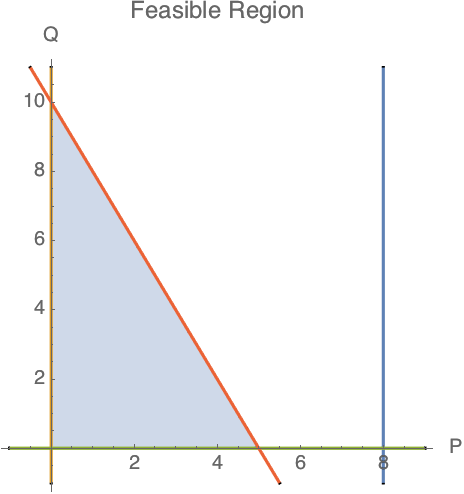
\includegraphics[scale=.7]{Figures/final_1}
        \end{center}
        Note that this problem can be expressed in two dimensions as $R$
        solely depends on $P$ and $Q$ and doesn't have any restrictions.
        Once $P$ and $Q$ are determined $R$ can be determined and the value of
        the objective function can be found.
        Since the objective function is linear, the optimal solution solution
        to this problem must lie on one of the corner points of the feasible
        region or there will be infinitely many optimal solutions along the
        border.
        Therefore I will first consider the 3 corner points of the feasible
        region.
        The first corner point $(0, 0)$ clearly has zero profit, as $P = 0$
        and $Q = 0$ so therefore $R = 0$ and $\v{c}^T \v{x} = 0$.
        At the second corner point $P = 5$ and $Q = 0$, so $R = 10$.
        In this case the profit will be $15 - 10\theta$.
        At the last corner point $Q = 10$ and $P = 0$, thus $R = 20$.
        In this case the profit will be $40 - 20\theta$.
        These two profits are linear with respect to $\theta$ and they are
        not parallel, so therefore there must be values of $\theta$ such that
        $40 - 20\theta > 15 - 10\theta$.
        This can be solved to give an interval on which the profit at $(0, 10)$
        is greater.
        \begin{align*}
          40 - 20\theta &> 15 - 10\theta \\
          35 &> 10\theta \\
          3.5 &> \theta \\
        \end{align*}
        When $\theta < 3.5$, then the profit at $Q = 10$ and $P = 0$ is greater.
        However note that for $\theta > 2$ the profit at $Q = 10$ and $P = 0$
        is negative as $40 - 20\theta = 0$ at $\theta = 2$.
        In this case when $\theta > 2$, then the optimal profit is at $P = 0$
        and $Q = 0$.
        This represents when the raw materials cost more than the value of the
        finished product.
        In this case it is best not to make any of the final product.
        So for $\theta < 2$ the optimal solution is $P = 0$, $Q = 10$, and
        $R = 20$.
        For $\theta > 2$ the optimal solution is $P = 0$, $Q = 0$, and
        $R = 0$.
    \end{enumerate}
\end{enumerate}
\end{document}
